\documentclass[a4paper, 11pt, oneside]{book}
\usepackage[utf8]{inputenc}
\usepackage[margin=3cm, bindingoffset=1cm]{geometry}
\usepackage[italian]{babel}
\usepackage{tikz}
\usepackage{svg}
\usepackage{array}
\usepackage[T1]{fontenc}
\usepackage{csquotes}
\linespread{1.7}
\usepackage{url}
\PassOptionsToPackage{hyphens}{url}
\usepackage{comment}
\usepackage[breaklinks]{hyperref}
\usepackage{float}
\usepackage{csquotes}
\usepackage{subfig}
\usepackage{graphicx}
\usepackage{afterpage}
\usepackage{fancyhdr}
\setlength{\parindent}{1cm}
\pagestyle{fancy}
\renewcommand{\chaptermark}[1]{\markboth{\thechapter.\ \uppercase{#1}}{}}
\fancyhf{}
\fancyhead[C]{\textbf{\leftmark}}
\fancyfoot[C]{\thepage}
\renewcommand{\headrulewidth}{1pt}
\renewcommand{\footrulewidth}{1pt}
\usepackage[Conny]{fncychap}

\usepackage[demo]{graphicx}
\usepackage{caption}
\usepackage{subcaption}
\usepackage{listings}
\usepackage{lmodern}  % for bold teletype font
\usepackage{amsmath}  % for \hookrightarrow
\usepackage{tabularx}
\usepackage[backend=bibtex, style=authortitle-comp, natbib=true]{biblatex}
\addbibresource{bib.bib}

\lstset{
  basicstyle=\ttfamily,
  columns=fullflexible,
  frame=single,
  breaklines=true,
  postbreak=\mbox{\textcolor{red}{$\hookrightarrow$}\space},
}

\usepackage{xcolor}

\definecolor{codegreen}{rgb}{0,0.6,0}
\definecolor{codegray}{rgb}{0.5,0.5,0.5}
\definecolor{codepurple}{rgb}{0.58,0,0.82}
\definecolor{backcolour}{rgb}{0.95,0.95,0.92}
\definecolor{verdino}{HTML}{00AE45}
\definecolor{biancosporco}{rgb}{245,245,245}

\lstdefinestyle{mystyle}{
    backgroundcolor=\color{backcolour},   
    commentstyle=\color{codegray},
    keywordstyle=\color{magenta},
    numberstyle=\tiny\color{codegray},
    stringstyle=\color{codegreen},
    basicstyle=\ttfamily\footnotesize,
    breakatwhitespace=false,         
    breaklines=true,                 
    captionpos=b,                    
    keepspaces=true,                 
    numbers=left,                    
    numbersep=5pt,                  
    showspaces=false,                
    showstringspaces=false,
    showtabs=false,                  
    tabsize=2
}

\lstset{style=mystyle}


\title{Appunti}
\author{}
\date{}

\newenvironment{dedication}
  {\clearpage           % we want a new page
   \thispagestyle{empty}% no header and footer
   \vspace*{\stretch{1}}% some space at the top 
   \itshape             % the text is in italics
   \raggedleft          % flush to the right margin
  }
  {\par % end the paragraph
   \vspace{\stretch{3}} % space at bottom is three times that at the top
   \clearpage           % finish off the page
  }
  
  
  
\newcommand\summaryname{Abstract}
\newenvironment{Abstract}%
    {\small\begin{center}%
    \bfseries{\summaryname} \end{center}}
    
\newcommand\blankpage{%
    \null
    \thispagestyle{empty}%
    \addtocounter{page}{-1}%
    \newpage}
  
\renewcommand\lstlistingname{Codice}
\renewcommand\lstlistlistingname{Elenco dei codici}  
  
  
\begin{document}
% Frontespizio
\begin{titlepage}
    \begin{center}
        \LARGE{\uppercase{\textbf{Università degli Studi di Salerno}}}\\
        \vspace{5mm}
        % Dipartimento
        \fontsize{15}{14}\selectfont{\uppercase{Dipartimento di INFORMATICA}}\\
    \end{center}
    \begin{figure}[H]
        \centering
        
\includegraphics[width=0.45\textwidth]{immagini/logo_standard.png}
    \end{figure}
    
    \begin{center}
    	%Titolo
        {\LARGE{\bf PROGRAMMAZIONE WEB}}\\
        \fontsize{15}{14}\selectfont{\textbf{Website Design}}
    	\vspace{5mm}
    \end{center}

    \begin{center}
        {\Large \bfseries ``DinoStore''}
    \end{center}
   
\noindent\begin{minipage}[t]{8cm}
\flushleft
\textsc{Docente}

Prof. \textbf{Gennaro Costagliola} \\
Prof. \textbf{Mattia De Rosa} \\
\end{minipage}
%
\hfill
%
\begin{minipage}[t]{6cm}
\flushright
\textsc{Studenti}

\textbf{Sorridi Generoso} \\
Matricola: 05121 16784

\textbf{Speranza Giuseppe} \\
Matricola: 05121 16601

\textbf{Zaino Alessandra} \\
Matricola: 05121 16280
\end{minipage}


    
    \vspace{15mm}
    \noindent
    
    \vspace{20mm}
    
\centering    
\normalsize Anno Accademico 2023-2024

\end{titlepage}


%Corpo della Tesi
\tableofcontents
\clearpage
\sloppy
\hyphenpenalty=10000
\exhyphenpenalty=10000



%--------------------------------------------------------------------------------
%	CHAPTER 1
%--------------------------------------------------------------------------------

\chapter{OBIETTIVO DEL PROGETTO}

Il nostro e-commerce DinoStore, è rivolto agli amanti dei dinosauri domestici offrendo una vasta gamma di prodotti dedicati a questi magnifici animali preistorici. Non solo vogliamo soddisfare le esigenze dei nostri clienti, ma vogliamo anche alimentare la loro passione per questi affascinanti creature offrendo l'opportunità di ospitare un vero dinosauro domestico.
\\
DinoStore propone tutto il necessario per accogliere e prendersi cura del vostro dinosauro domestico. Inoltre, assicura di fornire informazioni dettagliate su ciascun prodotto e di garantire una piattaforma di acquisto sicura e user-friendly per una esperienza di shopping senza problemi.
\\
Il nostro obiettivo principale è rendere l'esperienza di acquisto presso DinoStore facile e divertente per tutti i nostri clienti. Vogliamo essere il luogo di riferimento per gli appassionati di dinosauri domestici offrendo solo prodotti di alta qualità.



%--------------------------------------------------------------------------------
%	CHAPTER 2
%--------------------------------------------------------------------------------

\chapter{ANALISI DI SITI ESISTENTI}
\section{Everything Dinosaur}
\href{https://www.everythingdinosaur.com/}{\textbf{everythingdinosaur.com}}
\\
Un negozio online specializzato in giocattoli, modellini e articoli educativi legati ai dinosauri. Offrono una vasta selezione di prodotti e sono conosciuti per la loro attenzione ai dettagli scientifici.
\\
\textbf{Sito da browser web:}
\begin{figure}[H]
        \centering
        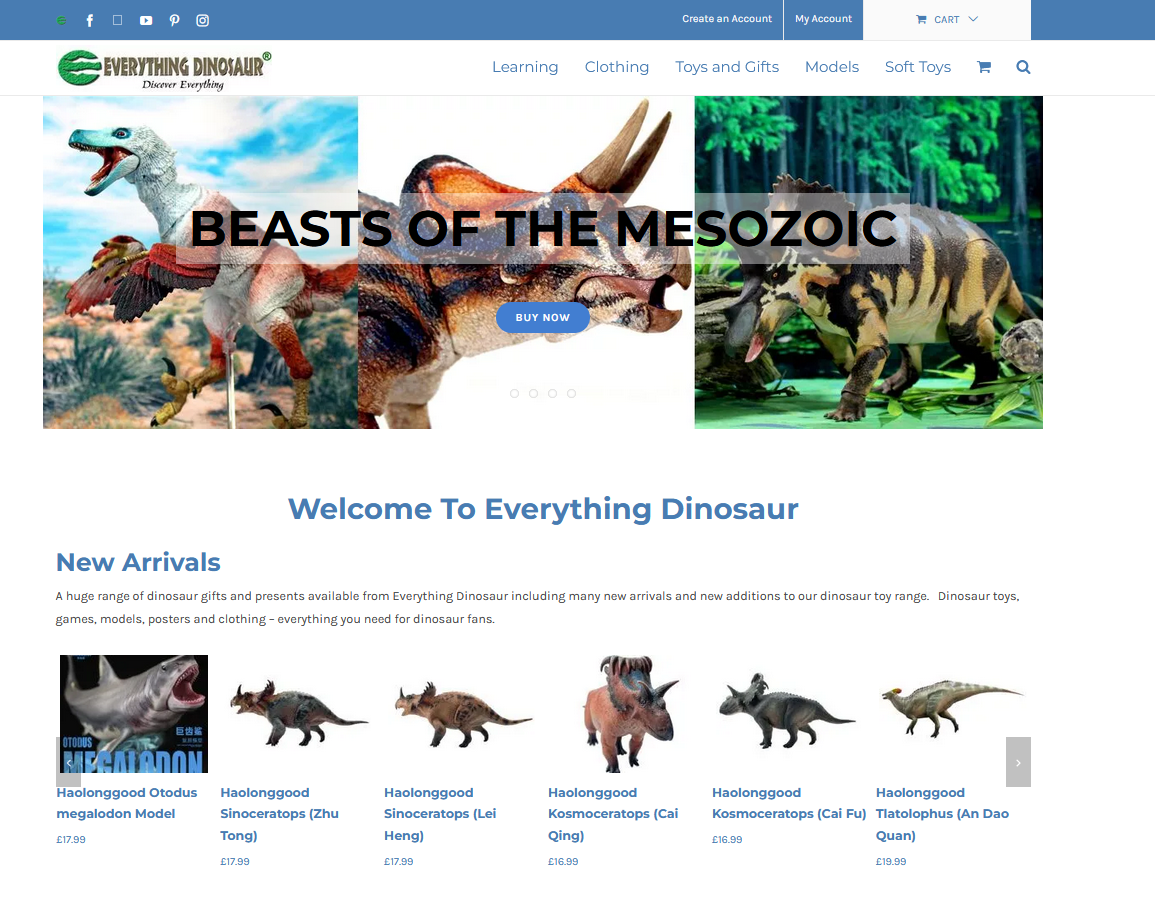
\includegraphics[width=0.60\textwidth]{immagini/everythingdinosaurpng.png}
        \caption{Everything dinosaur visualizzazione da desktop}
    \end{figure}
    
\textbf{Sito da mobile:}
\begin{figure}[H]
        \centering
        
\includegraphics[width=0.45\textwidth]{immagini/everythingdinosaur_mobile.jpg}
        \caption{Everything dinosaur visualizzazione da mobile}
    \end{figure}

Il sito si presenta con un'interfaccia semplice, anche se non molto intuitiva. L'header è composto dai contatti e dal logo del sito web, mentre nella parte destra è possibile creare un account, effettuare il login e visualizzare il carrello. Gli utenti non registrati, possono esplorare il sito e visualizzare i prodotti, ma hanno accesso limitato a funzionalità avanzate come il salvataggio degli articoli nel carrello per un accesso futuro. Tuttavia possono effettuare un ordine e procedere al check-out senza dover necessariamente creare un profilo.
\\
Nel corpo del sito troviamo un carosello composto da tre immagini con scorrimento manuale. Nella parte inferiore destra troviamo varie categorie, come articoli da regalo, vestiti, modellini, e una lente d'ingrandimento per cercare prodotti all'interno del sito. Scorrendo ulteriormente, troviamo un carosello di prodotti con i nuovi arrivi e i vari modellini suddivisi in base alle caratteristiche distintive di ogni dinosauro. Ogni prodotto ha una pagina dedicata con una descrizione dettagliata, immagini di alta qualità e informazioni aggiuntive come dimensioni, materiali e altre caratteristiche pertinenti. 
\\
Nel footer notiamo invece varie informazioni relative alla storia del sito stesso e i motivi per cui acquistare sul loro ecommerce. Più in basso troviamo la possibilità di iscriversi alla newsletter. 

\begin{figure}[H]
        \centering
        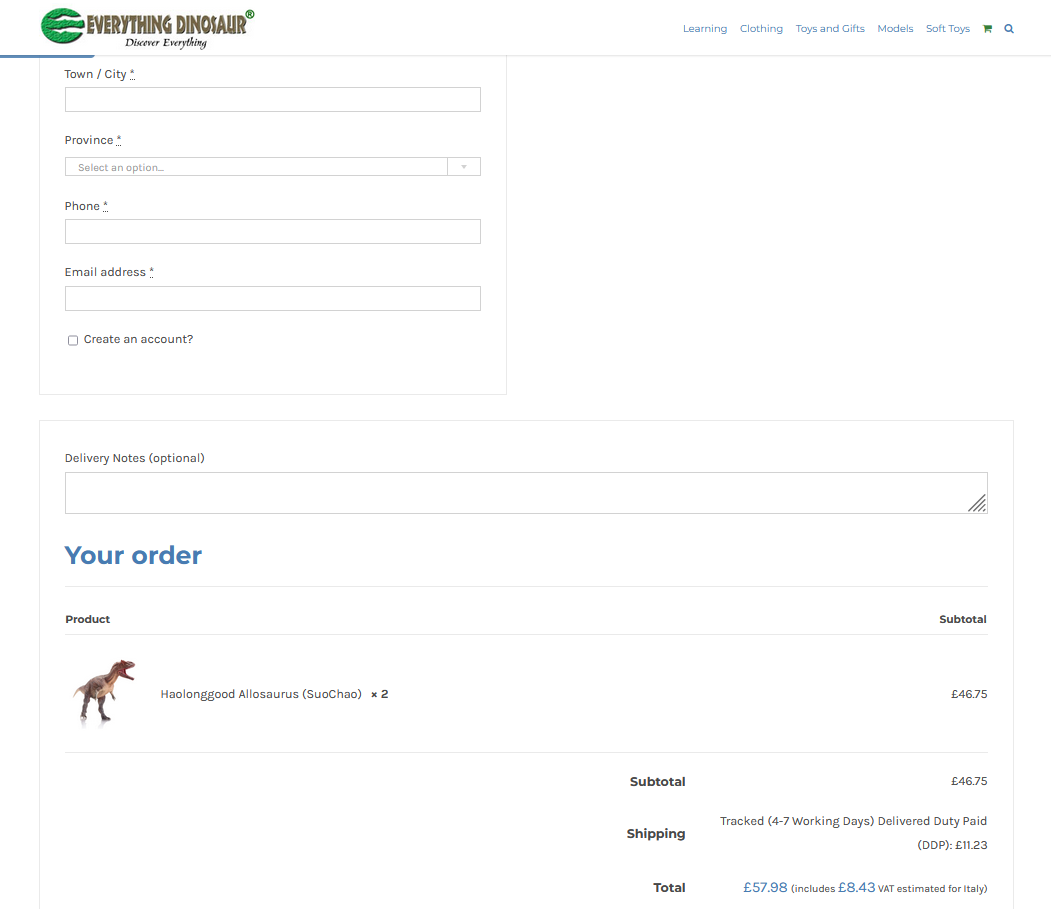
\includegraphics[width=0.80\textwidth]{immagini/everything_dinosaur_checkout.png}
        \caption{Check-out everything dinosaur}
    \end{figure}
\section{Dinosaur Corporation}
\href{https://www.dinosaurcorporation.com/}{\textbf{dinosaurcorporation.com}}
\\Dinosaur Corporation è un sito specializzato nella vendita di prodotti correlati ai dinosauri che offre una vasta selezione di giocattoli, peluche, modellini e articoli da collezione legati a questi animali. Le informazioni sono dettagliate, il servizio clienti è affidabile e le opzioni di pagamento sono sicure per soddisfare le esigenze dei suoi clienti. 
\\
\textbf{Sito da browser web:}
\begin{figure}[H]
        \centering
        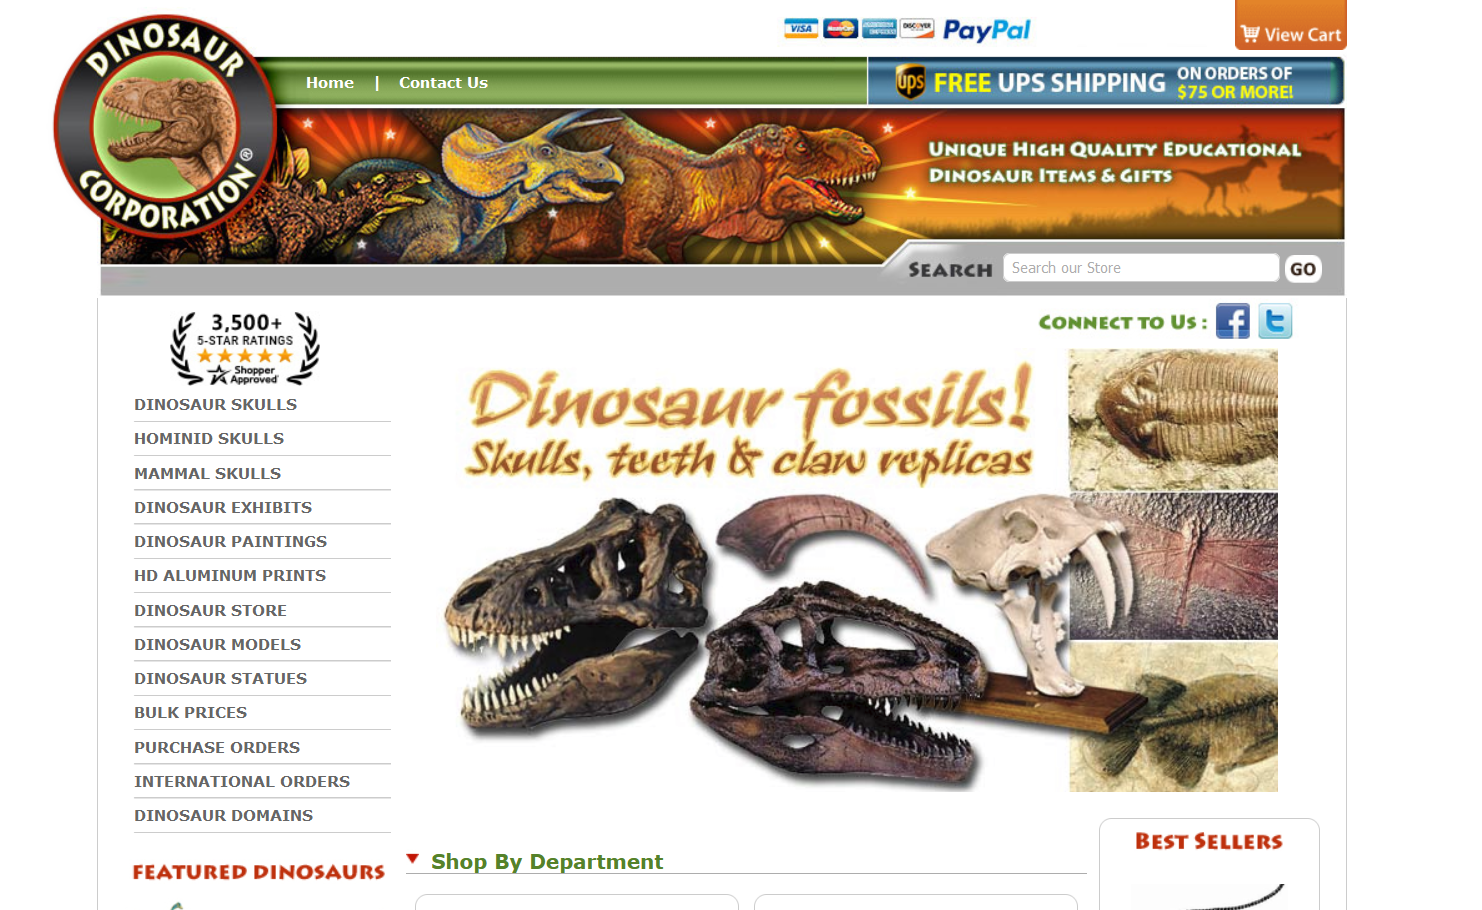
\includegraphics[width=0.60\textwidth]{immagini/dinosaurcorporation.png}
        \caption{Dinosaur corporation visualizzazione web}
    \end{figure}

\textbf{Sito da mobile:}
\begin{figure}[H]
        \centering
        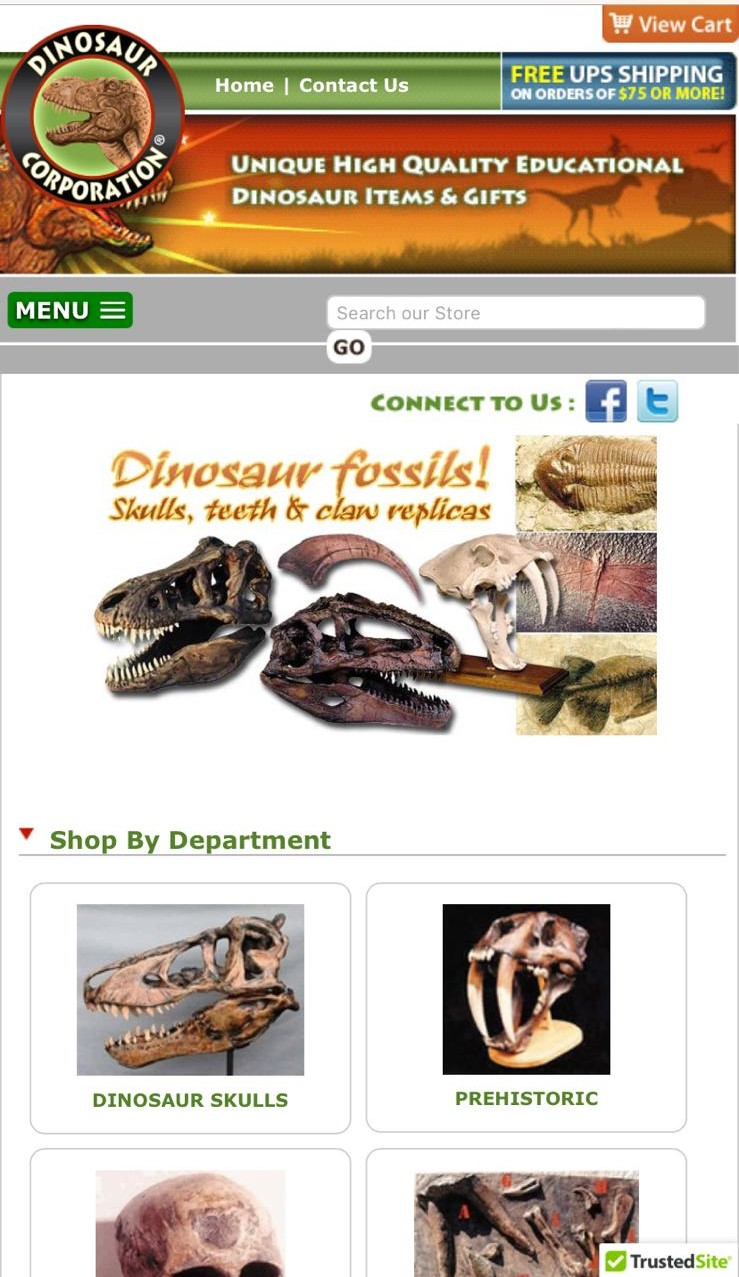
\includegraphics[width=0.45\textwidth]{immagini/dinosaurcorporation_mobile.jpg}
        \caption{Dinosaur Corporation visualizzazione da mobile}
    \end{figure}
L’homepage del sito si presenta con un’interfaccia meno moderna e per questa ragione alcuni utenti potrebbero avere difficoltà ad accedere ai prodotti offerti. Nell’header superiore è presente il logo del sito, i contatti e a destra abbiamo la possibilità di vedere il carrello. Più in basso troviamo una barra di ricerca con la quale possiamo navigare tra i vari prodotti del sito. Nella homepage troviamo i prodotti suddivisi in diverse categorie, ognuna delle quali ha un'immagine rappresentativa. Selezionando una categoria troviamo tutti i prodotti relativi a quest'ultima e la possibilità di aggiungerli direttamente al carrello. In questo sito web non è possibile effettuare una registrazione o un log-in. La schermata del carrello è la seguente, dove possiamo visualizzare la lista dei prodotti e i relativi prezzi, eventualmente possiamo vedere anche il prezzo della spedizione. 
\begin{figure}[H]
        \centering
        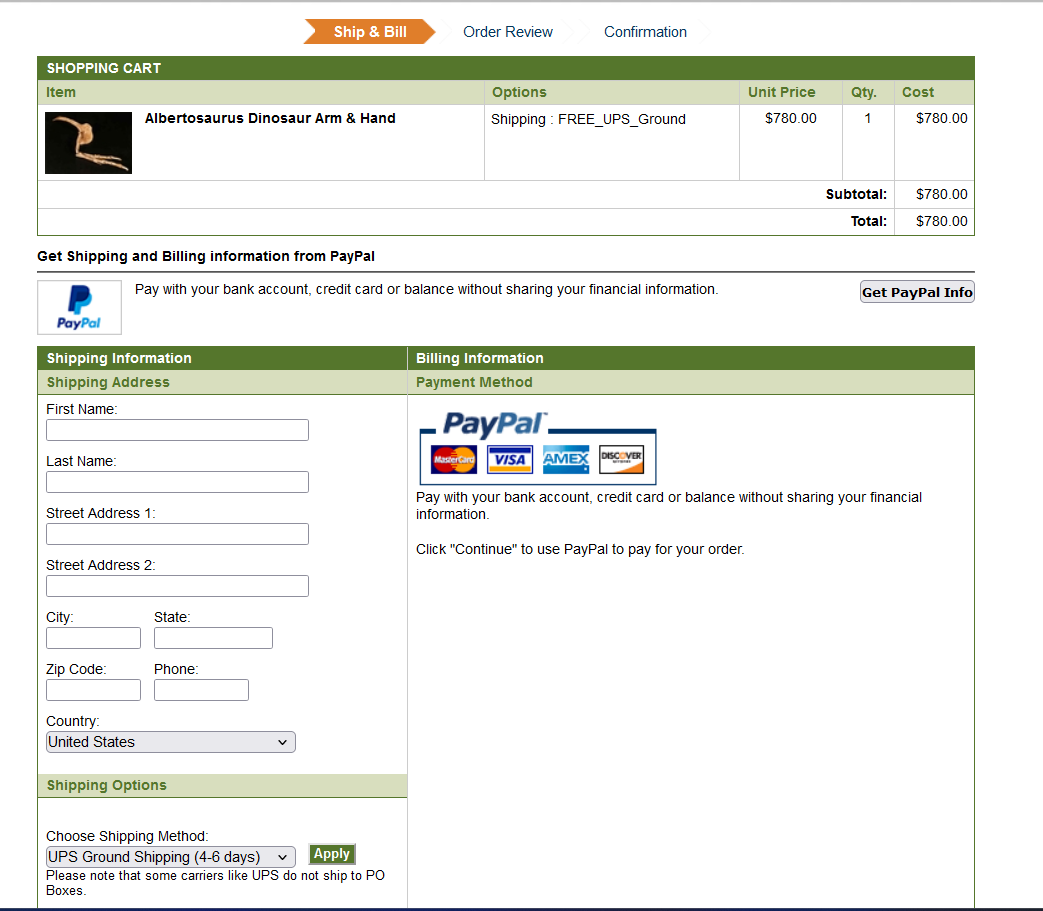
\includegraphics[width=0.70\textwidth]{immagini/dinosaur_corporation_checkout.png}
        \caption{Check-out di Dinosaur Corporation }
    \end{figure}
    
\section{Rocco Giocattoli}
\href{https://shop.roccogiocattoli.eu/brand/jurassic-world}{\textbf{roccogiocattoli.eu/brand/jurassic-world}}
\\
Rocco Giocattoli è un negozio online specializzato in modellini di Jurassic World. Il sito si presenta con un'interfaccia semplice visualizzando un header che mostra in alto a sinistra il logo, al centro una barra di ricerca per navigare all'interno del sito e a destra il carrello e l'area utente.
\\
L'homepage parte con la presentazione dei vari prodotti in catalogo e la possibilità di aggiungerli al carrello o alla lista desideri, il menù è suddiviso in varie categorie di prodotti. Inoltre è possibile filtrare tramite la barra laterale il prezzo e l'età consigliata dei vari giocattoli. 
\\
Nel footer, invece, troviamo informazioni sulle spedizioni, i pagamenti, i contatti, la storia dell'azienda e un altro collegamento all'area utente.
\\

\textbf{Sito da browser web:}
\begin{figure}[H]
        \centering
        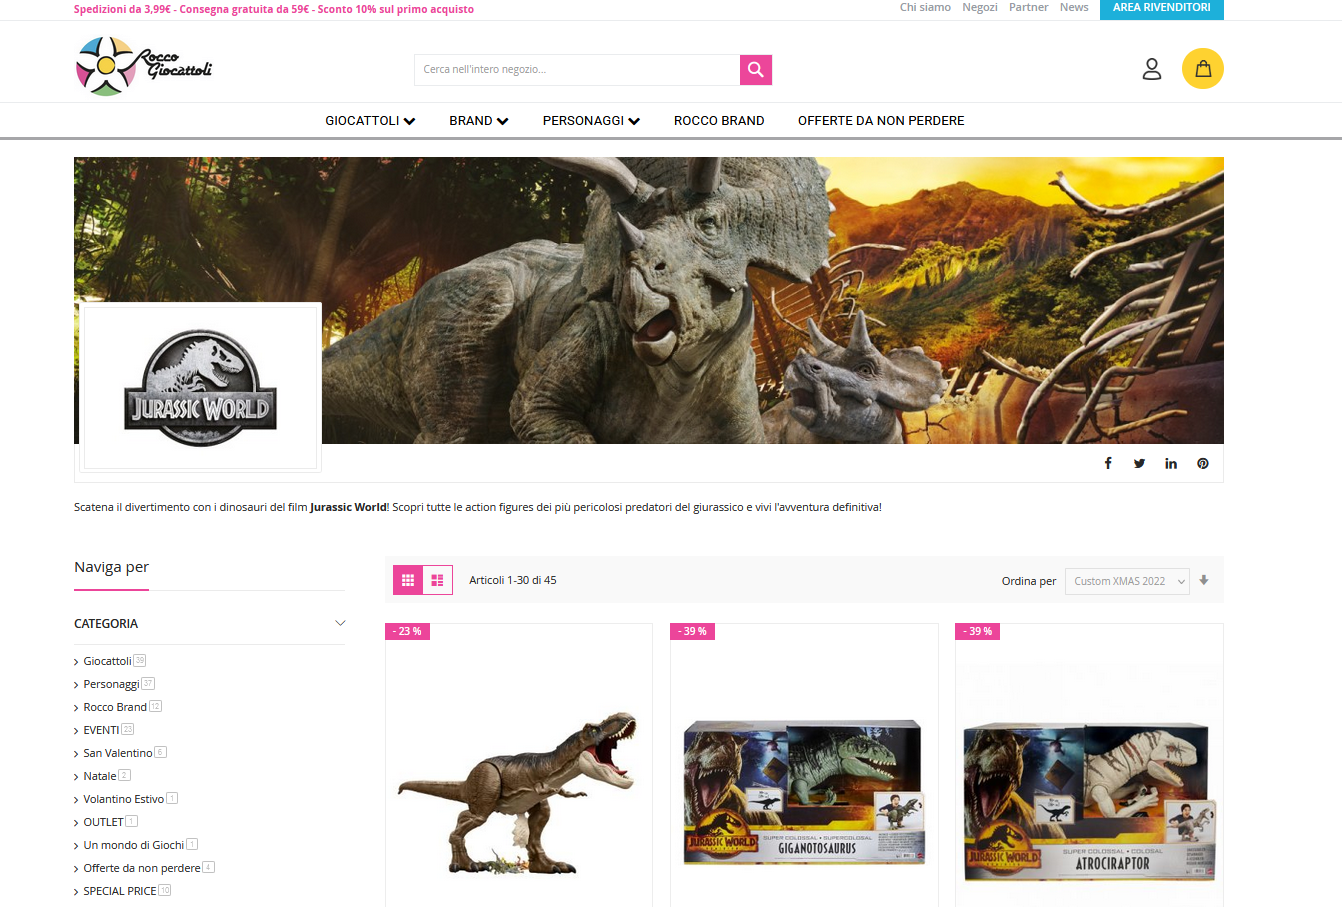
\includegraphics[width=0.50\textwidth]{immagini/roccogiocattoli.png}
        \caption{Rocco Giocattoli visualizzazione da browser web}
    \end{figure}
    
\textbf{Sito da mobile:}
\begin{figure}[H]
        \centering
        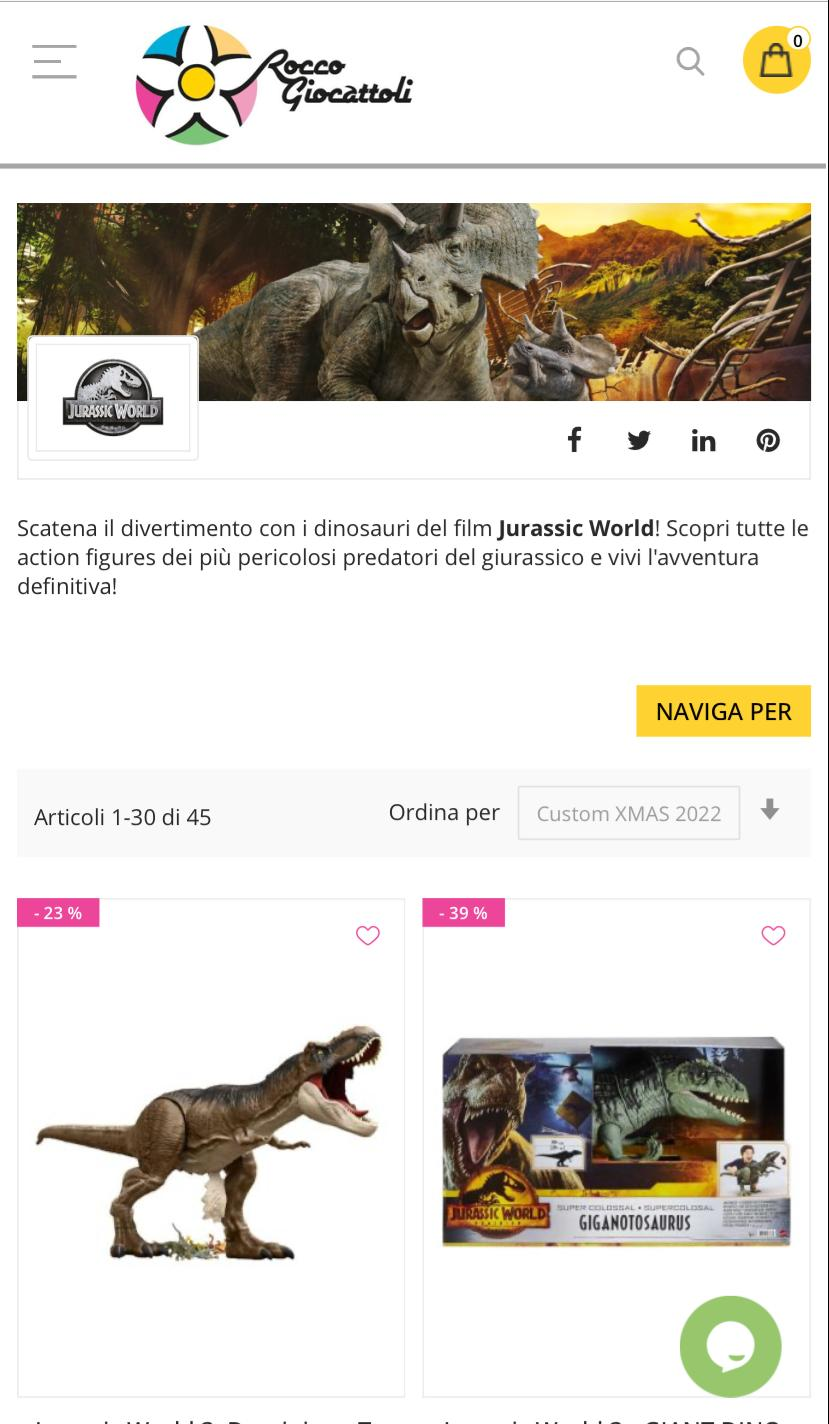
\includegraphics[width=0.35\textwidth]{immagini/roccogiocattoli_mobile.jpg}
        \caption{Rocco Giocattoli visualizzazione del sito da mobile}
    \end{figure}
Selezionando un prodotto da acquistare abbiamo la possibilità di scegliere se aggiungerlo al carrello, comprarlo subito o aggiungerlo ad un'eventuale lista dei desideri, e varie informazioni tra cui tempi di consegna e caratteristiche dell'articolo. è anche possibile lasciare una recensione, non bisogna essere registrati ne tanto meno aver fatto l'acquisto del prodotto specifico. 
\begin{figure}[H]
        \centering
        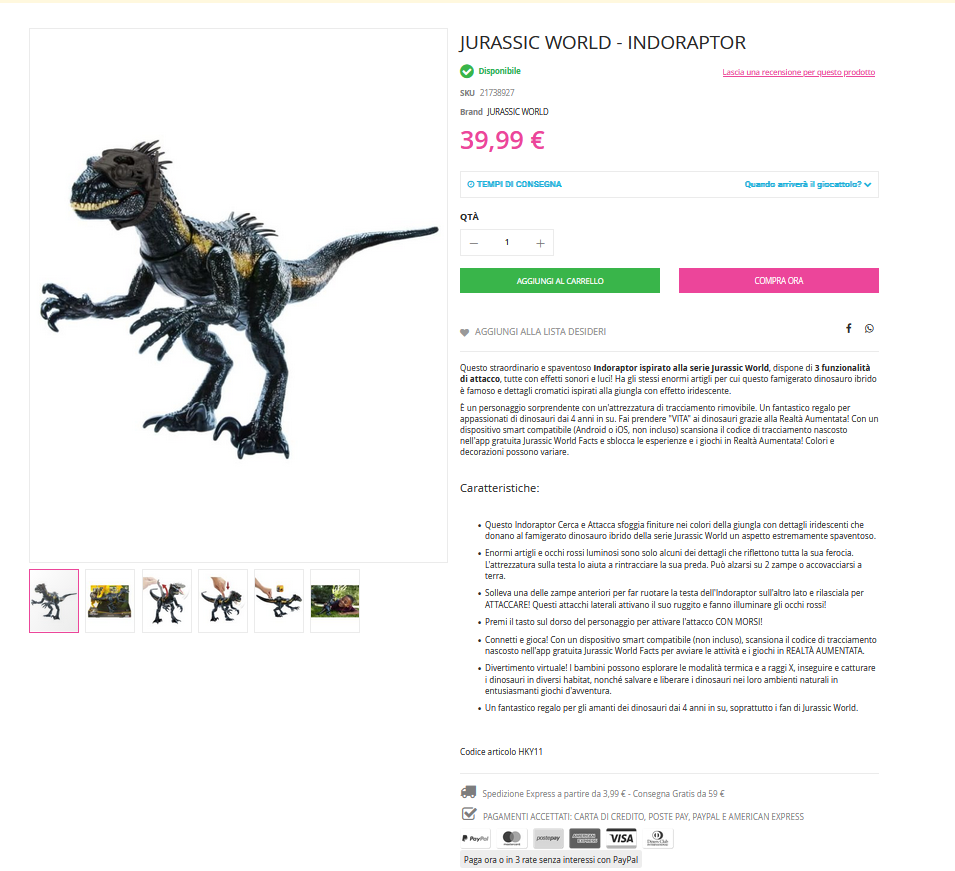
\includegraphics[width=0.5\textwidth]{immagini/prodotto_roccogiocattoli.png}
        \caption{Pagina del prodotto }
    \end{figure}
Il cliente può aggiungere prodotti al carrello senza necessariamente essere registrato o aver fatto il login, procedendo al check-out compare la seguente schermata:
 \begin{figure}[H]
        \centering
        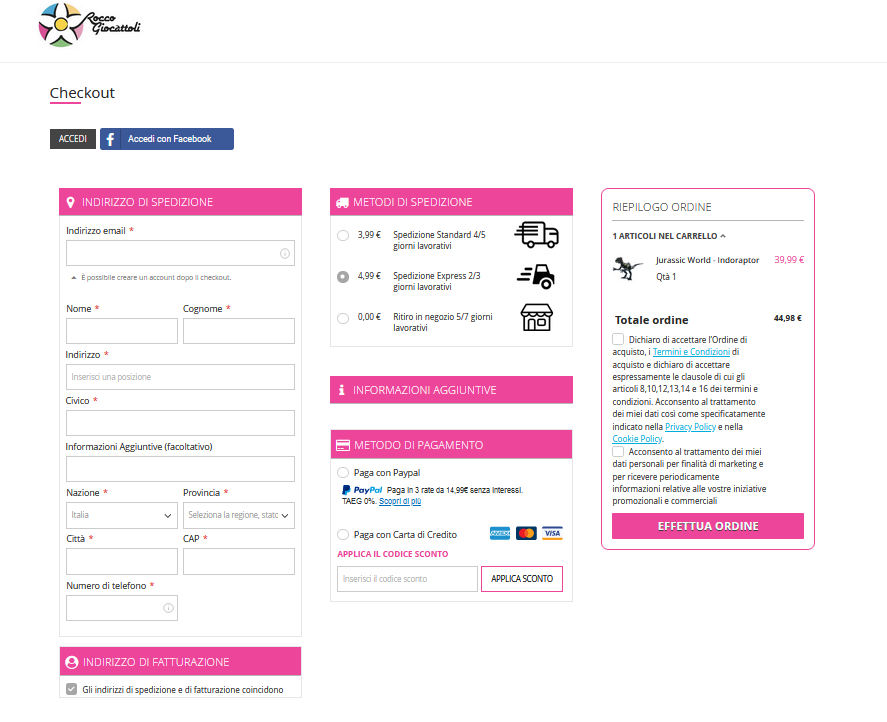
\includegraphics[width=0.55\textwidth]{immagini/check-out_roccogiocattoli.png}
        \caption{Check-out Rocco Giocattoli}
    \end{figure}
Nella sezione carrello anche se non si è registrati è possibile visualizzare la lista dei prodotti inseriti e il totale che comprende anche la spedizione.

\begin{comment}
    Il sito proposto `e un e-commerce specializzato nella vendita di dinosauri domestici,
mirato a un pubblico di appassionati di animali insoliti e originali. La piattaforma
si propone di soddisfare i bisogni dei clienti interessati all’acquisto di dinosauri
domestici come animali da compagnia o come oggetti di collezione. Offrir`a una
vasta gamma di prodotti relativi ai dinosauri, fornendo informazioni dettagliate sui
prodotti e facilitando il processo di acquisto attraverso un’interfaccia user-friendly
e sicura.
\end{comment}



%--------------------------------------------------------------------------------
%	CHAPTER 3
%--------------------------------------------------------------------------------

\chapter{FUNZIONALITÀ DEL SITO}
% sistemiamo la documentazione. (sono animali da collezione o da compagnia?)
\paragraph{Il nostro sito di e-commerce dedicato ai dinosauri domestici, uova, ossa fossili e guinzagli offre una serie di funzionalità progettate per migliorare l'esperienza di shopping sia per gli utenti che per gli amministratori. Gli utenti possono godere di opzioni avanzate di ricerca e di filtraggio, facilitando la scoperta e l'acquisto dei loro dinosauri preferiti senza la necessità di un login per aggiungere al carrello. Gli amministratori hanno a disposizione strumenti sofisticati per gestire il catalogo di prodotti e monitorare le vendite.}

\section{Funzionalità per l'utente}
\begin{itemize}
    \item \textbf{Ricerca avanzata}: Una barra di ricerca che consente agli utenti di cercare dinosauri domestici tramite parole chiave.
    \item \textbf{Filtri di ricerca}: Opzioni di filtraggio per aiutare gli utenti a restringere i risultati della ricerca in base a criteri specifici come prezzo, categoria ecc...
    \item \textbf{Visualizzazione dei prodotti}: Gli utenti possono visualizzare i dinosauri domestici disponibili con dettagli completi come immagini, descrizioni, prezzi, ecc...
    \item \textbf{Carrello degli acquisti}: Un'area dedicata dove gli utenti possono visualizzare i prodotti che hanno aggiunto al carrello, modificare le quantità o procedere al pagamento.
\end{itemize}

\section{Funzionalità per l'amministratore}
\begin{itemize}
    \item \textbf{Aggiornamenti dell'inventario}: Funzionalità che consentono agli amministratori di monitorare l'inventario dei dinosauri domestici disponibili e di apportare eventuali aggiornamenti quando necessario.
    \item \textbf{Gestione dei prezzi}: Possibilità per gli amministratori di impostare prezzi competitivi per i dinosauri domestici e di apportare modifiche quando necessario.
    \item \textbf{Gestione delle descrizioni dei prodotti}: Capacità per gli amministratori di scrivere descrizioni dettagliate e accattivanti per i dinosauri domestici per informare e attirare gli acquirenti.
\end{itemize}

\section{Funzionalità per utente senza log in}
\begin{itemize}
    \item \textbf{Aggiungere e rimuovere prodotti nel carrello}: Gli utenti guest possono selezionare i prodotti desiderati e aggiungerli al carrello per un'ulteriore revisione o acquisto. Hanno anche la flessibilità di rimuovere articoli dal carrello se necessario.
    \item \textbf{Possibilità di Registrarsi}: Gli utenti hanno l'opzione di registrarsi per creare un account sul sito, consentendo loro di accedere a funzionalità avanzate e migliorare l'eseprienza complessiva di acquisto.
    \item \textbf{Funzione di ricerca prodotti}: Una funzione di ricerca consente agli utenti guest di trovare rapidamente i prodotti desiderati, semplificando il processo di navigazione e facilitando l'accesso ai contenuti pertinenti.
    \item \textbf{Richiesta di registrazione per acquisti}: Durante il checkout, agli utenti guest potrebbe essere richiesto di registrarsi.
\end{itemize}


%--------------------------------------------------------------------------------
%	CHAPTER 4
%--------------------------------------------------------------------------------

\chapter{DIAGRAMMA NAVIGAZIONALE}
\begin{figure}[H]
    \centering
    %\includesvg[width=0.5\textwidth]{immagini/Schema_Navigazionale}
    \caption{Schema Navigazionale del nostro sito web}
    \label{fig:svg_image}
\end{figure}



%--------------------------------------------------------------------------------
%	CHAPTER 5
%--------------------------------------------------------------------------------

\chapter{LAYOUT}
%da modificare
La struttura del layout web è stata progettata seguendo questi criteri:
\begin{itemize}
    \item Il \textbf{logo} è stato collocato nell'angolo in alto a sinistra.
    \item Delle \textbf{immagini a scorrimento} sono state inserite per illustrare lo scopo del sito, ossia la vendita di dinosauri e prodotti ad essi correlati.
    \item Un \textbf{menu di navigazione}  posto in alto al centro è stato organizzato per facilitare la selezione di prodotti.
    \item Nel corpo del sito troviamo sulla sinistra i vari \textbf{filtri} per semplificare la ricerca. Accanto possiamo trovare alcuni degli \textbf{articoli} presenti sull'e-commerce. 
    \item Il \textbf{footer} conterrà informazioni di contatto e altre utili risorse.
\end{itemize}
  \begin{figure}[H]
        \centering
        
\includegraphics[width=0.80\textwidth]{immagini/desktop_view.png}
        \caption{Visione desktop dell'e-commerce}
    \end{figure}


%--------------------------------------------------------------------------------
%	CHAPTER 6
%--------------------------------------------------------------------------------

%\chapter{SCELTA DEI COLORI }
I \textbf{colori} principali del sito saranno:
\\
%ho messo colori a caso dopo i primi due
 
\begin{tikzpicture}
  \fill[verdino, draw=black] (0,0) rectangle (3,3);
  \node[text width=0.7\textwidth, align=justify, anchor=west] at (3.2,1.5) {\textcolor{verdino}{00AE46:} Il colore 00ae46 è un verde vivace che evoca natura e vitalità. Perfetto per un sito che vende dinosauri, offre un legame con l'habitat preistorico dei dinosauri, suggerisce crescita e rinascita, fornisce un contrasto visivo accattivante e attrae il pubblico giovane.};
\end{tikzpicture}
\\

\begin{tikzpicture}
\fill[white, draw=black] (0,0) rectangle (3,3);
\node[text width=0.7\textwidth, align=justify, anchor=west] at (3.2,1.5) {\textcolor{black}{FFFFFF:} Il bianco, associato a pulizia, semplicità ed eleganza, è un'ottima scelta per un sito che vende dinosauri. Trasmette chiarezza e mette in risalto i prodotti, offrendo anche versatilità nell'aggiunta di elementi di design.};
\end{tikzpicture}
\\

\begin{comment}
\begin{tikzpicture}
    \fill[biancosporco, draw=black] (0,0) rectangle (3,3);
    \node[text width=0.7\textwidth, align=justify, anchor=west] at (3.2,1.5) {\textcolor{black}{F5F5F5:} };
    \end{tikzpicture}    
\end{comment}



%--------------------------------------------------------------------------------
%	CHAPTER 6
%--------------------------------------------------------------------------------

\chapter{SCELTA DEI COLORI }
I \textbf{colori} principali del sito saranno:
\\
%ho messo colori a caso dopo i primi due
 
\begin{tikzpicture}
  \fill[verdino, draw=black] (0,0) rectangle (3,3);
  \node[text width=0.7\textwidth, align=justify, anchor=west] at (3.2,1.5) {\textcolor{verdino}{00AE46:} Il colore 00ae46 è un verde vivace che evoca natura e vitalità. Perfetto per un sito che vende dinosauri, offre un legame con l'habitat preistorico dei dinosauri, suggerisce crescita e rinascita, fornisce un contrasto visivo accattivante e attrae il pubblico giovane.};
\end{tikzpicture}
\\

\begin{tikzpicture}
\fill[white, draw=black] (0,0) rectangle (3,3);
\node[text width=0.7\textwidth, align=justify, anchor=west] at (3.2,1.5) {\textcolor{black}{FFFFFF:} Il bianco, associato a pulizia, semplicità ed eleganza, è un'ottima scelta per un sito che vende dinosauri. Trasmette chiarezza e mette in risalto i prodotti, offrendo anche versatilità nell'aggiunta di elementi di design.};
\end{tikzpicture}
\\

\begin{comment}
\begin{tikzpicture}
    \fill[biancosporco, draw=black] (0,0) rectangle (3,3);
    \node[text width=0.7\textwidth, align=justify, anchor=west] at (3.2,1.5) {\textcolor{black}{F5F5F5:} };
    \end{tikzpicture}    
\end{comment}



%--------------------------------------------------------------------------------
%	CHAPTER 7
%--------------------------------------------------------------------------------

%\chapter{MAPPA DEI CONTENUTI}



%--------------------------------------------------------------------------------
%	CHAPTER 8
%--------------------------------------------------------------------------------

\chapter{BASE DI DATI}
\begin{figure}[H]
        \centering
        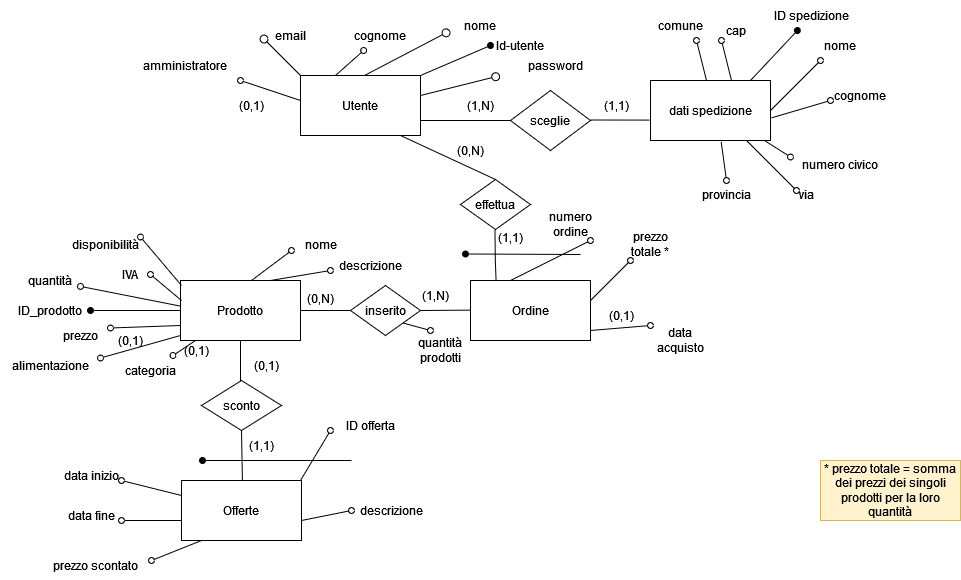
\includegraphics[width=1.0\textwidth]{immagini/Schema_ER_progetto_tsw(1).drawio(1).png}
        \caption{Schema ER}
    \end{figure}




\clearpage
\nocite{*}
\raggedright
\clearpage
\listoffigures
\addcontentsline{toc}{chapter}{\listfigurename}
\clearpage



\end{document}

